\documentclass{article}
\usepackage[utf8]{inputenc}
\usepackage{graphicx}
\usepackage{float}
\title{CS251 Report}
\author{Arpit Gupta }
\date{26 March 2018}

\begin{document}

\maketitle

Hi Check out my assignment below!\\
Enjoy!\\
\section{Graph}
\begin{figure}[H]
    \centering
    \includegraphics[scale=.5]{sca1.eps}
    \caption{Scattering Graph1}
    \label{fig:my_label}
\end{figure}
This is the first scattering graph !\\
Go on\\
\section{Graph}
\begin{figure}[H]
    \centering
    \includegraphics[scale=.5]{sca2.eps}
    \caption{Scattering Graph1}
    \label{fig:my_label}
\end{figure}
This is the second scattering graph !\\
Go on\\
\section{Graph}
\begin{figure}[H]
    \centering
    \includegraphics[scale=.5]{sca4.eps}
    \caption{Scattering Graph1}
    \label{fig:my_label}
\end{figure}
This is the third scattering graph !\\
Go on\\
\section{Graph}
\begin{figure}[H]
    \centering
    \includegraphics[scale=.5]{sca8.eps}
    \caption{Scattering Graph1}
    \label{fig:my_label}
\end{figure}
This is the fourth scattering graph !\\
Go on\\
\section{Graph}
\begin{figure}[H]
    \centering
    \includegraphics[scale=.5]{sca16.eps}
    \caption{Scattering Graph1}
    \label{fig:my_label}
\end{figure}
This is the fifth scattering graph !\\
Go on\\
\section{Graph}
\begin{figure}[H]
    \centering
    \includegraphics[scale=.5]{aver.eps}
    \caption{Linear Graph1}
    \label{fig:my_label}
\end{figure}
This is the average line graph !\\
Go on\\
\section{Graph}
\begin{figure}[H]
    \centering
    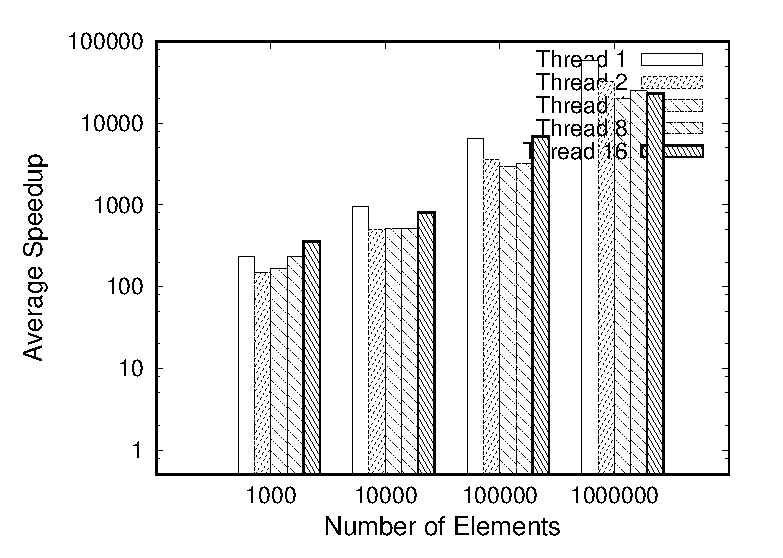
\includegraphics[scale=.5]{speedup.eps}
    \caption{histogram}
    \label{fig:my_label}
\end{figure}
This is the speed up histogram !\\
Go on\\
\section{Graph}
\begin{figure}[H]
    \centering
    \includegraphics[scale=.5]{Variance.eps}
    \caption{histogram}
    \label{fig:my_label}
\end{figure}
This is the Variance Histogram !\\
Bye \\
Have a nice day!\\



\end{document}
